\chapter{Printed Circuit Board Design Fundamentals}\label{ch:pcb}

\begin{tipbox}[When to Read This Chapter]
\textbf{Sprint~3}: Read the full chapter if your project includes a custom PCB. The design must be frozen at CDR to allow 4--6 weeks for fabrication and bring-up. \textbf{Sprint~4}: Use the bring-up protocol and visual inspection checklist when your boards arrive. \textbf{Dev board projects}: Skim the grounding, decoupling, and trace width sections; these principles apply to breadboard wiring too. \textbf{Related}: Circuit theory in Chapter~13 (p.\,\pageref{ch:electronics}); power architecture in Chapter~12 (p.\,\pageref{ch:power}); ESP32 pin assignments in Chapter~19 (p.\,\pageref{ch:mcu}); debugging in Chapter~20 (p.\,\pageref{ch:debug}).
\end{tipbox}

\vspace{1em}
\section{PCB Structure and Materials}

A printed circuit board is a layered sandwich of insulating substrate (FR-4 fiberglass-epoxy) with patterned copper conductors. Copper traces, pads, and planes are created by chemically etching unwanted copper from a continuous sheet. A \textbf{solder mask} (the green coating) protects copper from oxidation and shorts. A \textbf{silkscreen\index{silkscreen}} layer prints component outlines and reference designators.

\begin{figure}[htbp]\centering
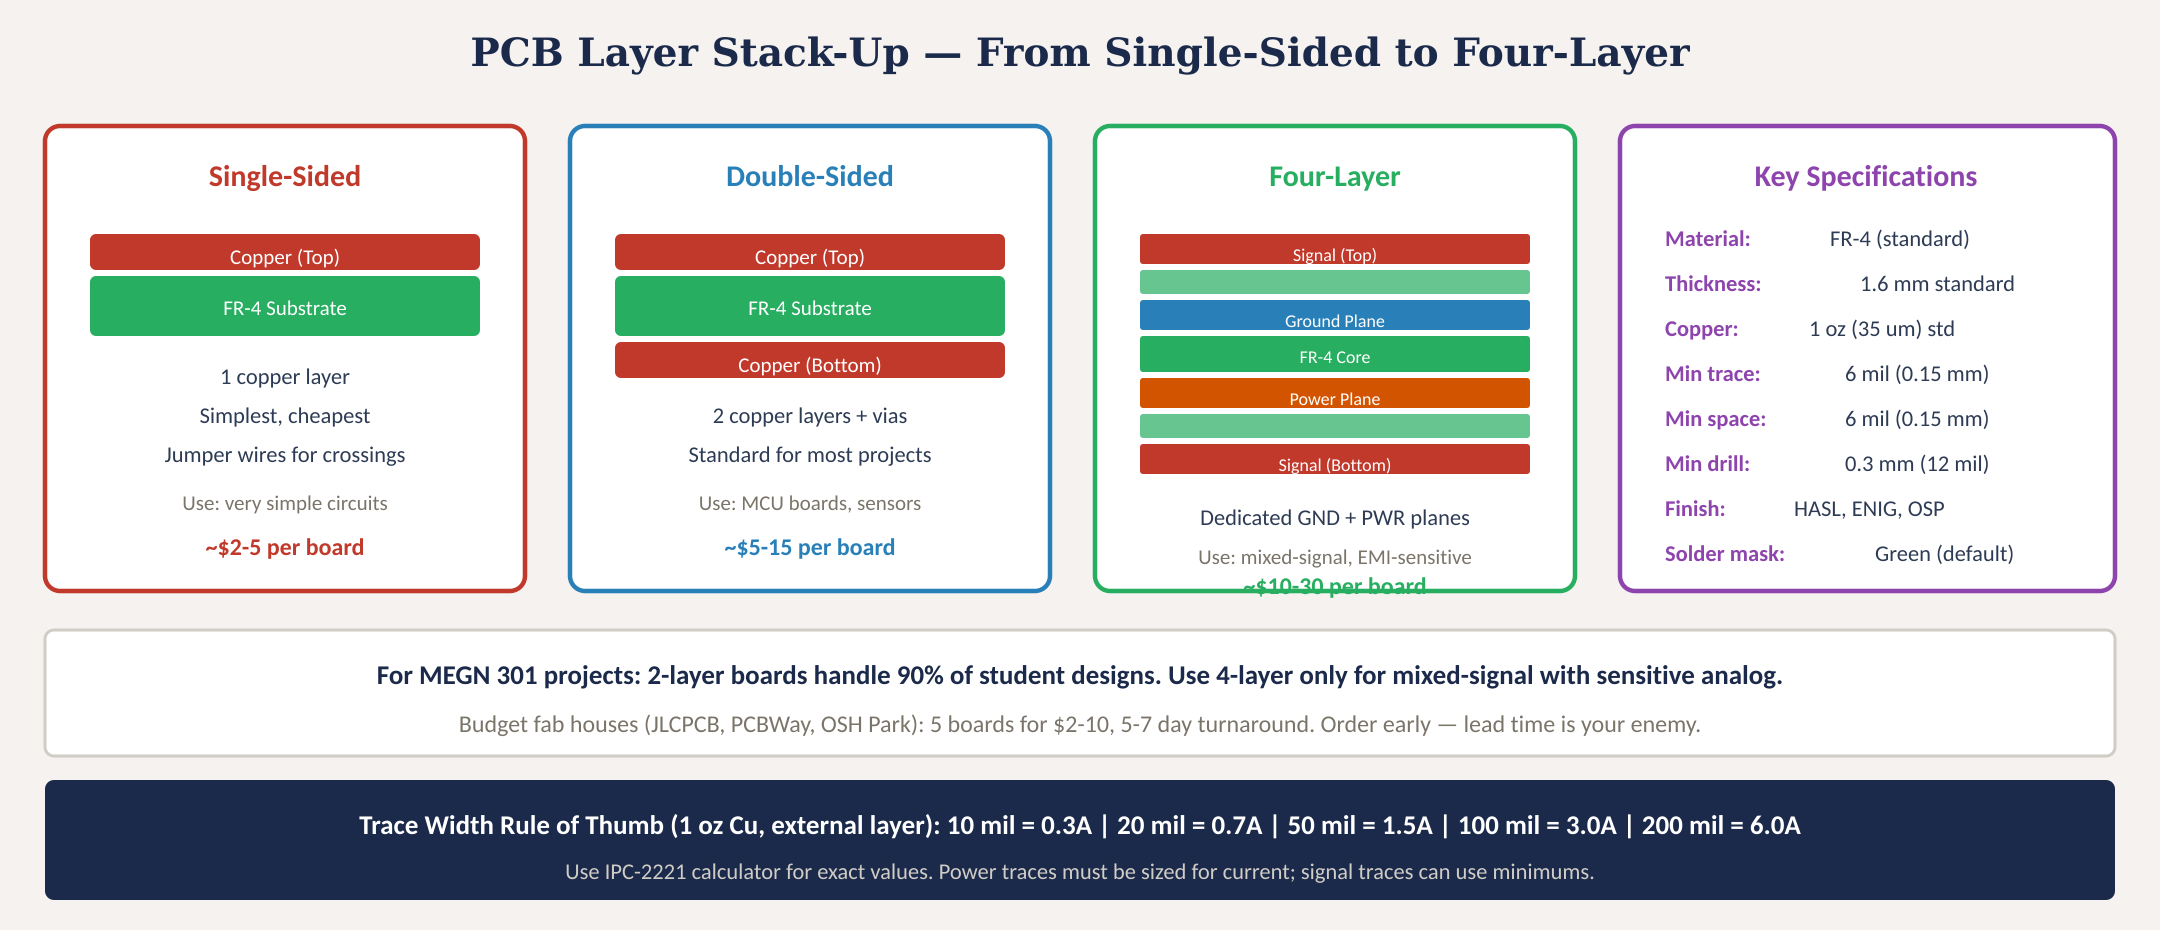
\includegraphics[width=\textwidth]{master_figs/fig_pcb_layer_stackup.png}
\caption{PCB layer stack-ups from single-sided to four-layer with key specifications and trace width\index{trace width (PCB)} current reference.}\label{fig:stack}
\end{figure}

\subsection{Layer Stack-Ups}
\textbf{Single-sided}: one copper layer. Simplest, cheapest (\$2--5). Jumper wires for crossings. Very simple circuits only. \textbf{Double-sided}: copper on both sides connected by vias (plated through-holes). Standard for 90\% of student projects (\$5--15). \textbf{Four-layer}: adds dedicated ground and power planes between signal layers. Use for mixed-signal or EMI-sensitive designs (\$10--30).

\subsection{Key Specifications}
FR-4 substrate, 1.6\,mm standard thickness, 1\,oz (35\,$\mu$m) copper, 6\,mil minimum trace/space, 0.3\,mm minimum drill. Surface finishes: HASL (cheapest, good for THT), ENIG (flat pads, good for SMD), OSP (organic, short shelf life).

\begin{warningbox}[Trace Width for Current]
A 10-mil trace on 1-oz external copper safely carries only 0.3\,A. Power traces must be sized for actual current: 10\,mil\,=\,0.3\,A, 20\,mil\,=\,0.7\,A, 50\,mil\,=\,1.5\,A, 100\,mil\,=\,3.0\,A, 200\,mil\,=\,6.0\,A. Use the IPC-2221\index{IPC-2221} calculator for exact values. Signal traces can use minimums; power traces must be sized for current.
\end{warningbox}

\subsection{Component Packages}

\begin{figure}[htbp]\centering
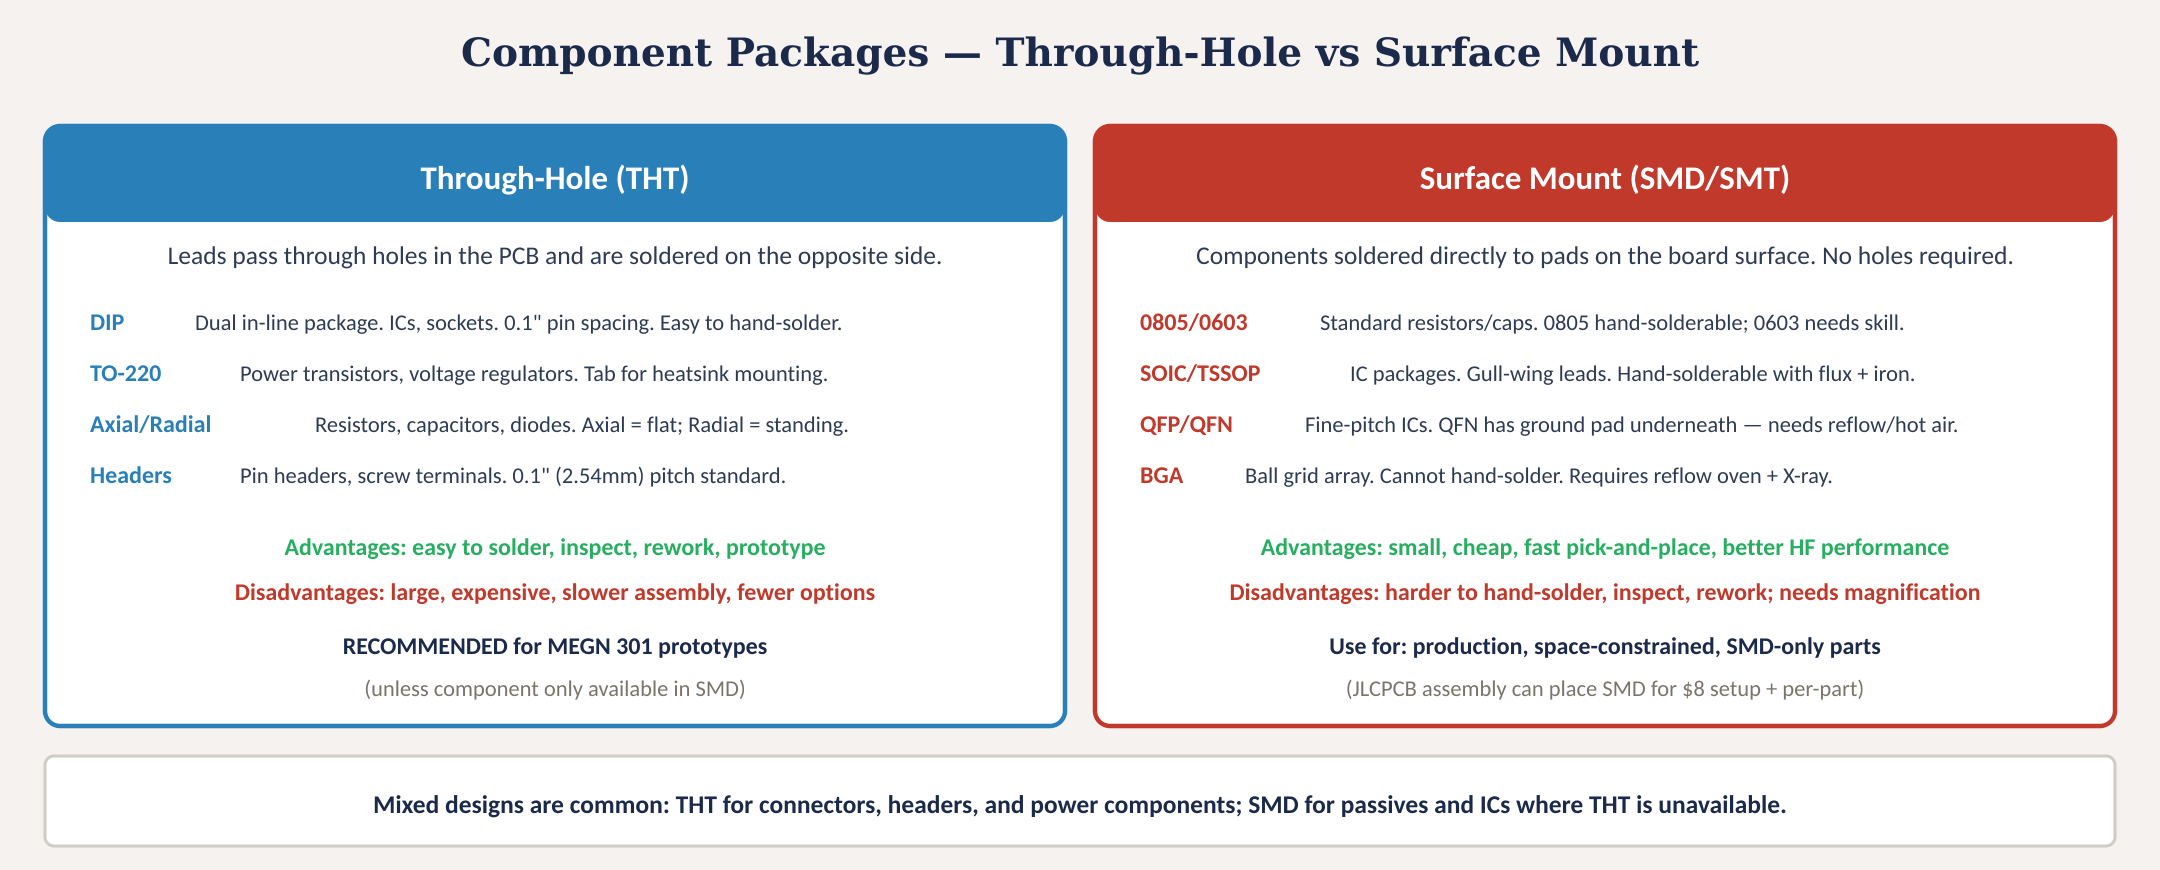
\includegraphics[width=\textwidth]{master_figs/fig_pcb_component_packages.png}
\caption{Through-hole vs surface-mount packages with common types and soldering guidance.}\label{fig:pkg}
\end{figure}

\textbf{Through-hole (THT)}: leads pass through holes. DIP, TO-220, axial/radial, pin headers. Easy to hand-solder, inspect, and rework. Recommended for MEGN 301 prototypes. \textbf{Surface-mount (SMD/SMT)}: soldered to pads on the board surface. 0805/0603 passives, SOIC/TSSOP ICs, QFP/QFN fine-pitch. Smaller, cheaper, but harder to hand-solder. Use SMD only when THT is unavailable or space is critical. Mixed designs are common.

\section{Design Workflow}

\begin{figure}[htbp]\centering
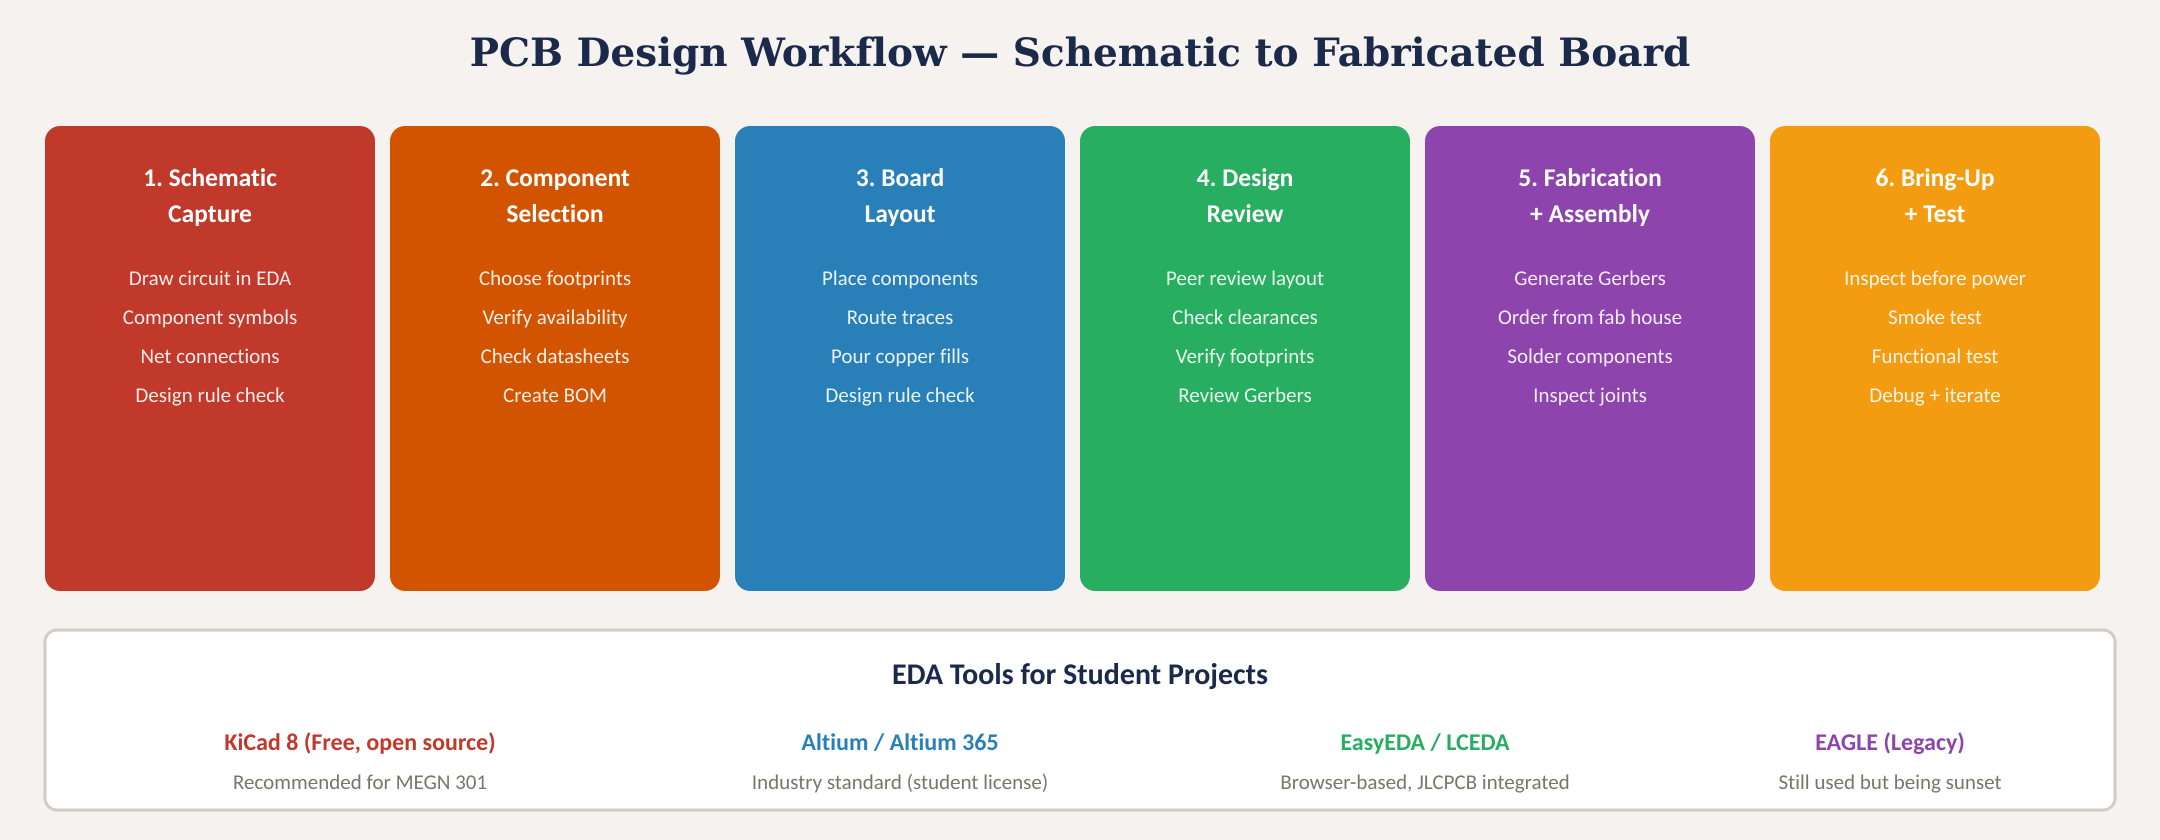
\includegraphics[width=\textwidth]{master_figs/fig_pcb_design_workflow.png}
\caption{Six-stage PCB design workflow from schematic capture\index{schematic capture} through board bring-up.}\label{fig:wkfl}
\end{figure}

Six stages: (1) \textbf{Schematic capture}; draw circuit with component symbols and net connections. (2) \textbf{Component selection}; map symbols to physical footprints, verify availability, create BOM. (3) \textbf{Board layout}; place components, route traces, pour copper fills. (4) \textbf{Design review}; peer review, check clearances, verify footprints, review Gerbers\index{Gerber files}. (5) \textbf{Fabrication + assembly}; generate Gerbers, order boards, solder. (6) \textbf{Bring-up + test}; inspect, smoke test, functional test, debug.

Recommended EDA tool: \textbf{KiCad\index{KiCad} 8} (free, open-source, fully capable). Alternatives: Altium (industry standard, student license), EasyEDA (browser-based, JLCPCB\index{JLCPCB} integrated).


\section{Schematic Capture Best Practices}

\subsection{Schematic Organization}
A professional schematic is a \emph{communication document}, not just a wiring diagram. Follow these rules from IPC-2612 [20]:
\begin{enumerate}[nosep,leftmargin=1.5em]
\item \textbf{One functional block per sheet}: power supply on Sheet~1, MCU + peripherals on Sheet~2, motor drivers on Sheet~3, connectors on Sheet~4. Title each sheet.
\item \textbf{Signal flow left to right}: inputs on the left, outputs on the right. Power flows top (VCC) to bottom (GND).
\item \textbf{Net labels over long wires}: replace wires that cross the entire sheet with named net labels (e.g., \texttt{MOTOR\_PWM}, \texttt{SDA}, \texttt{VBAT}). This eliminates spaghetti routing.
\item \textbf{Power flags}: explicitly show where power enters the schematic. Add decoupling caps adjacent to every IC symbol, not on a separate ``capacitor page.''
\item \textbf{Consistent reference designators}: R for resistors, C for capacitors, U for ICs, J for connectors, D for diodes, Q for transistors, L for inductors.
\end{enumerate}

\subsection{Component Selection and Footprint Verification}\index{footprint verification}
The most expensive PCB mistake is a wrong footprint. For every component:
\begin{enumerate}[nosep,leftmargin=1.5em]
\item Download the \textbf{manufacturer's datasheet} (not a distributor summary page).
\item Find the \textbf{recommended land pattern} (footprint) in the datasheet's ``Package Information'' section.
\item Verify the KiCad library footprint dimensions match the datasheet \textbf{exactly}: pad size, pad pitch, courtyard.
\item If no library footprint exists, create one from the datasheet using KiCad's footprint editor. Measure twice.
\item \textbf{Cross-check}: print the footprint at 1:1 scale and physically place the component on the printout.
\end{enumerate}

\begin{warningbox}[The \$50 Footprint Mistake]
A team ordered 5 PCBs (\$25 total) with a QFN-32 footprint that had the wrong pad pitch (0.5\,mm vs.\ 0.65\,mm). All 5 boards were scrap. The fix required a new board spin: another \$25 + 2 weeks of lost schedule. Total cost of one unchecked footprint: \$50 + 2 weeks. The 1:1 printout would have caught this in 30 seconds.
\end{warningbox}

\subsection{Design Rule Configuration}
Configure KiCad's DRC rules before starting layout:
\begin{table}[htbp]\centering\small
\begin{tabularx}{\textwidth}{l c c X}
\toprule
\textbf{Rule} & \textbf{Minimum} & \textbf{Recommended} & \textbf{Notes} \\
\midrule
Trace width (signal) & 6\,mil & 10\,mil & Wider = easier to solder rework \\
Trace width (power) & Per IPC calc & 50--200\,mil & Size for actual current \\
Trace spacing & 6\,mil & 8\,mil & Tight spacing increases fab cost \\
Via drill & 0.3\,mm & 0.4\,mm & Smaller vias cost more \\
Via annular ring & 0.15\,mm & 0.25\,mm & Larger = more reliable \\
Clearance to edge & 0.3\,mm & 0.5\,mm & Prevents copper exposure at board edge \\
\bottomrule
\end{tabularx}
\caption{Recommended DRC rules for MEGN~301 PCBs (JLCPCB/PCBWay compatible).}
\end{table}

\section{Critical Layout Rules}

\begin{figure}[htbp]\centering
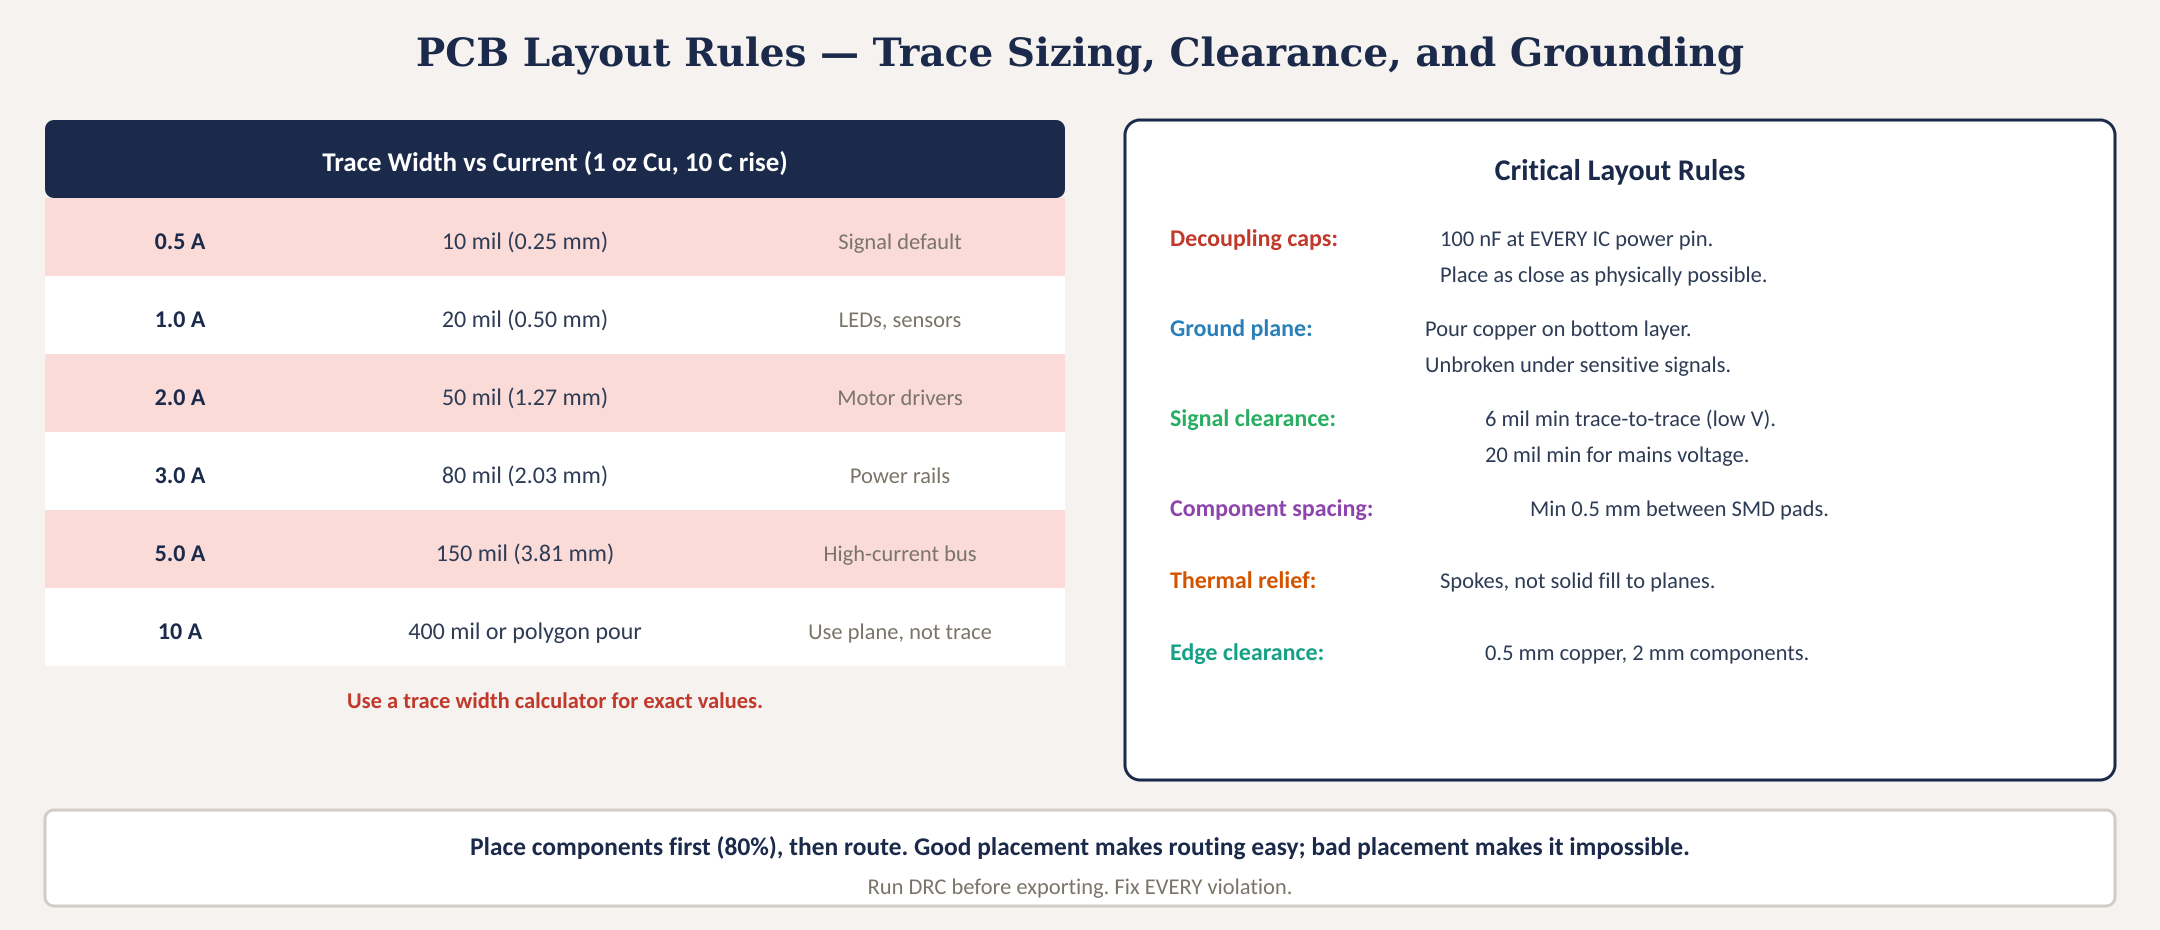
\includegraphics[width=\textwidth]{master_figs/fig_pcb_layout_rules.png}
\caption{PCB layout rules\index{PCB layout}: decoupling, ground planes, component placement, and routing priorities.}\label{fig:pcb_layout_rules}\end{figure}

\subsection{Decoupling Capacitors}
The critical layout rules are summarized in Figure~\ref{fig:pcb_layout_rules}. Place a 100\,nF ceramic capacitor within 5\,mm of every IC power pin, connected with the shortest possible traces. Add one 10\,$\mu$F bulk capacitor per power rail. Via directly to ground plane for the ground side. This is not optional; without decoupling, MCUs reset and ADCs produce garbage data.

\subsection{Ground Plane}\index{ground plane}
On a 2-layer board, fill the bottom layer with a ground copper pour. This provides a low-impedance return path for all signals and dramatically reduces noise. Connect the pour to GND with abundant vias. Avoid splitting the ground plane; a split forces return current to detour.

\subsection{Component Placement and Routing}
Place components before routing. Group by function. Keep high-current paths short. Route power first, then sensitive signals, then non-critical digital. Avoid 90-degree trace corners (use 45-degree). Keep analog and digital sections physically separated. Add thermal relief pads on ground-plane connections for hand soldering.

\begin{tipbox}[The \#1 Rule]
\textbf{PRINT YOUR BOARD AT 1:1 SCALE AND PLACE REAL COMPONENTS ON THE PRINTOUT} before ordering. This single step catches 80\% of footprint errors; the most expensive PCB mistake (wrong footprint = scrap board).
\end{tipbox}

\section{Fabrication, Assembly, and Bring-Up}

\subsection{Fabrication Files}
\textbf{Gerber files} (RS-274X format): one per layer. \textbf{Drill files} (Excellon): hole coordinates and diameters. \textbf{BOM + pick-and-place}: for assembly services. Always verify in a standalone Gerber viewer before ordering.

\subsection{Fab Houses}
JLCPCB: 5 boards for \$2--7 + shipping (5--7 day fab). PCBWay: similar. OSH Park: \$5/sq-in, US-based. Order early; total timeline is 4--6 weeks from design start to working board.

\subsection{Board Bring-Up Protocol}

\begin{warningbox}[Step 1 Is Mandatory: No Exceptions]
\textbf{Do not apply power to any board until Step~1 is complete and signed off.} Skipping visual inspection is the fastest way to destroy a \$40 ESP32 module. A single solder bridge\index{solder bridge} on a 0.5\,mm-pitch IC creates a dead short that damages the component the instant power is applied.
\end{warningbox}

\begin{enumerate}[leftmargin=1.5em]
\item \textbf{Visual inspection under $\geq$10$\times$ magnification} (loupe, USB microscope, or stereo microscope). This is a \textbf{mandatory gate}; a teammate must co-sign the inspection before power is applied. Inspect \emph{every} solder joint. Specific defects to look for:
\begin{itemize}[nosep,leftmargin=1.5em]
\item \textbf{Solder bridges}: look between adjacent pads on fine-pitch ICs (QFP, SOIC). A bridge shorts two pins.
\item \textbf{Cold joints}: dull, grainy, or blobby solder that did not wet the pad. These create intermittent connections.
\item \textbf{Tombstoned passives}: 0603/0805 components standing on one end (one pad soldered, one lifted).
\item \textbf{Missing components}: compare the board to the BOM and the schematic. Every refdes on the silkscreen should have a component.
\item \textbf{Wrong orientation}: check polarity marks on diodes, tantalum caps, ICs (pin 1 dot), and electrolytic caps.
\end{itemize}
\item \textbf{Continuity check}: multimeter between VCC and GND on every power rail. Any reading $<$10\,$\Omega$ indicates a short. \textbf{Do not proceed until all shorts are resolved.}
\item \textbf{Current-limited power}: set bench supply to expected voltage, current limit to 50\,mA. Apply power. If the supply immediately current-limits, there is a short. Remove power and re-inspect.
\item \textbf{Voltage verification}: measure every power rail with a multimeter. Each rail should read within $\pm$5\% of its nominal voltage.
\item \textbf{Smoke test}: increase current limit to the expected operating current. Monitor for 60 seconds. Watch for: components getting hot (touch-test cautiously), smell of burning flux or plastic, any visible smoke.
\item \textbf{Functional test}: load firmware, verify heartbeat LED, test each subsystem individually before connecting external hardware.
\end{enumerate}


\subsection{Design Review Checklist}
Before ordering PCBs, verify:
\begin{enumerate}[nosep,leftmargin=1.5em]
\item DRC (Design Rule Check) passes with zero errors and zero unreviewed warnings.
\item All footprints verified against component datasheets (not just library defaults).
\item Board outline correct with mounting holes matching the enclosure.
\item All connectors accessible and oriented correctly for cable routing.
\item Silkscreen readable (refdes near components, polarity marks on diodes/caps/ICs).
\item 1:1 printout with real components placed; \textbf{this catches 80\% of errors}.
\item Gerber files opened in a standalone viewer and visually inspected layer by layer.
\item BOM cross-checked against schematic (every schematic component in BOM and vice versa).
\item Peer review by at least one teammate who did not do the layout.
\end{enumerate}

\subsection{Development Board Integration}
When using a development board (ESP32 DevKit, Arduino Nano) instead of a custom PCB:
\begin{itemize}[nosep,leftmargin=1.5em]
\item Mount the dev board on a custom carrier PCB or perfboard with proper headers.
\item Use screw terminals or JST connectors (not breadboard jumper wires) for all permanent connections.
\item Add status LEDs and test points to the carrier board.
\item Document the wiring diagram with connector pin assignments.
\item Secure all wires with strain relief (zip ties, hot glue at connector exit points).
\end{itemize}
A well-wired development board that meets all requirements is superior to a custom PCB that delays the project or has errors.


\section{EMI, Noise, and Signal Integrity}

\subsection{The Return Current Problem}
Every signal current has a return current that flows through the ground plane (or ground trace) back to the source. The return current follows the path of \emph{least impedance}; at high frequencies, this is the path directly beneath the signal trace. If the ground plane is split or missing under a signal trace, the return current detours, creating a large loop antenna that radiates EMI and picks up noise.

\textbf{Rule}: never split the ground plane. If you must route a trace on the ground layer, stitch the ground pour\index{ground pour} back together with vias on both sides of the crossing.

\subsection{Analog-Digital Separation}
Mixed-signal boards (analog sensors + digital MCU + motor drivers) are the norm in MEGN~301 projects. Three strategies:
\begin{enumerate}[nosep,leftmargin=1.5em]
\item \textbf{Physical separation}: place analog components (sensors, ADC, analog filters) on one side of the board, digital components (MCU, motor drivers) on the other.
\item \textbf{Separate power rails}: use separate voltage regulators\index{voltage regulator} for analog and digital sections. At minimum, use an RC filter ($10\,\Omega + 10\,\mu$F) between the digital supply and the analog supply.
\item \textbf{Single-point ground connection}: if using split ground pours (advanced), connect them at exactly one point near the ADC. For most student projects, a single continuous ground pour with careful component placement is sufficient and safer.
\end{enumerate}

\subsection{Motor Noise Mitigation on PCB}
Motor PWM switching generates noise on every power and ground trace. Mitigation:
\begin{itemize}[nosep,leftmargin=1.5em]
\item Route motor power traces on a separate layer or board region from signal traces.
\item Place ceramic capacitors (100\,nF) directly across motor driver power pins.
\item Add a bulk electrolytic ($100$--$470\,\mu$F) at the motor power input.
\item Use a TVS diode on the motor power bus for transient suppression.
\item Never share ground vias between motor driver and MCU sections.
\end{itemize}

\section{Thermal Management on PCBs}
Components that dissipate significant power require thermal design:
\begin{itemize}[leftmargin=1.5em]
\item \textbf{Thermal pads}: many voltage regulators and motor drivers have an exposed pad on the bottom of the package. This pad \textbf{must} be soldered to a copper area on the PCB and connected to internal ground planes with thermal vias (array of 0.3\,mm vias on 1.0\,mm pitch under the pad).
\item \textbf{Copper pour as heatsink}: for SOT-223 or D-PAK regulators, extend the ground pour under and around the package. Each square centimeter of 1-oz copper on the outer layer provides approximately $60\,^{\circ}$C/W of thermal resistance to ambient.
\item \textbf{Thermal relief}: for hand-soldering, use thermal relief pads (spoke connections) on ground-connected pads. Without them, the ground plane wicks heat away faster than the soldering iron can supply it, resulting in cold joints\index{cold joint}.
\end{itemize}

\begin{tipbox}[Quick Thermal Check]
For any linear regulator: $P = (V_{in} - V_{out}) \times I_{load}$. If $P > 0.5$\,W, you need thermal analysis. If $P > 1$\,W, you probably need a switching regulator instead.
\end{tipbox}

\begin{keyconceptbox}[Requirements Mapping: From PCB Specs to Shall-Statements]
PCB design decisions directly generate system requirements:
\begin{itemize}[nosep,leftmargin=1.5em]
\item ``Board fits in 60$\times$40\,mm enclosure'' $\to$ SYS-REQ: The PCB shall have maximum dimensions of 58$\times$38\,mm with mounting holes at [coordinates].
\item ``Motor driver draws 3\,A'' $\to$ PCB-REQ: Motor power traces shall be $\geq$150\,mil wide on 1-oz copper.
\item ``ADC reads 0--3.3\,V sensors'' $\to$ PCB-REQ: Analog input traces shall be routed $\geq$10\,mm from motor power traces with a continuous ground plane beneath.
\end{itemize}
Every technical specification in Part~II should trace back to a shall-statement in your SDRD.
\end{keyconceptbox}

\section{Common Mistakes}

\begin{figure}[htbp]\centering
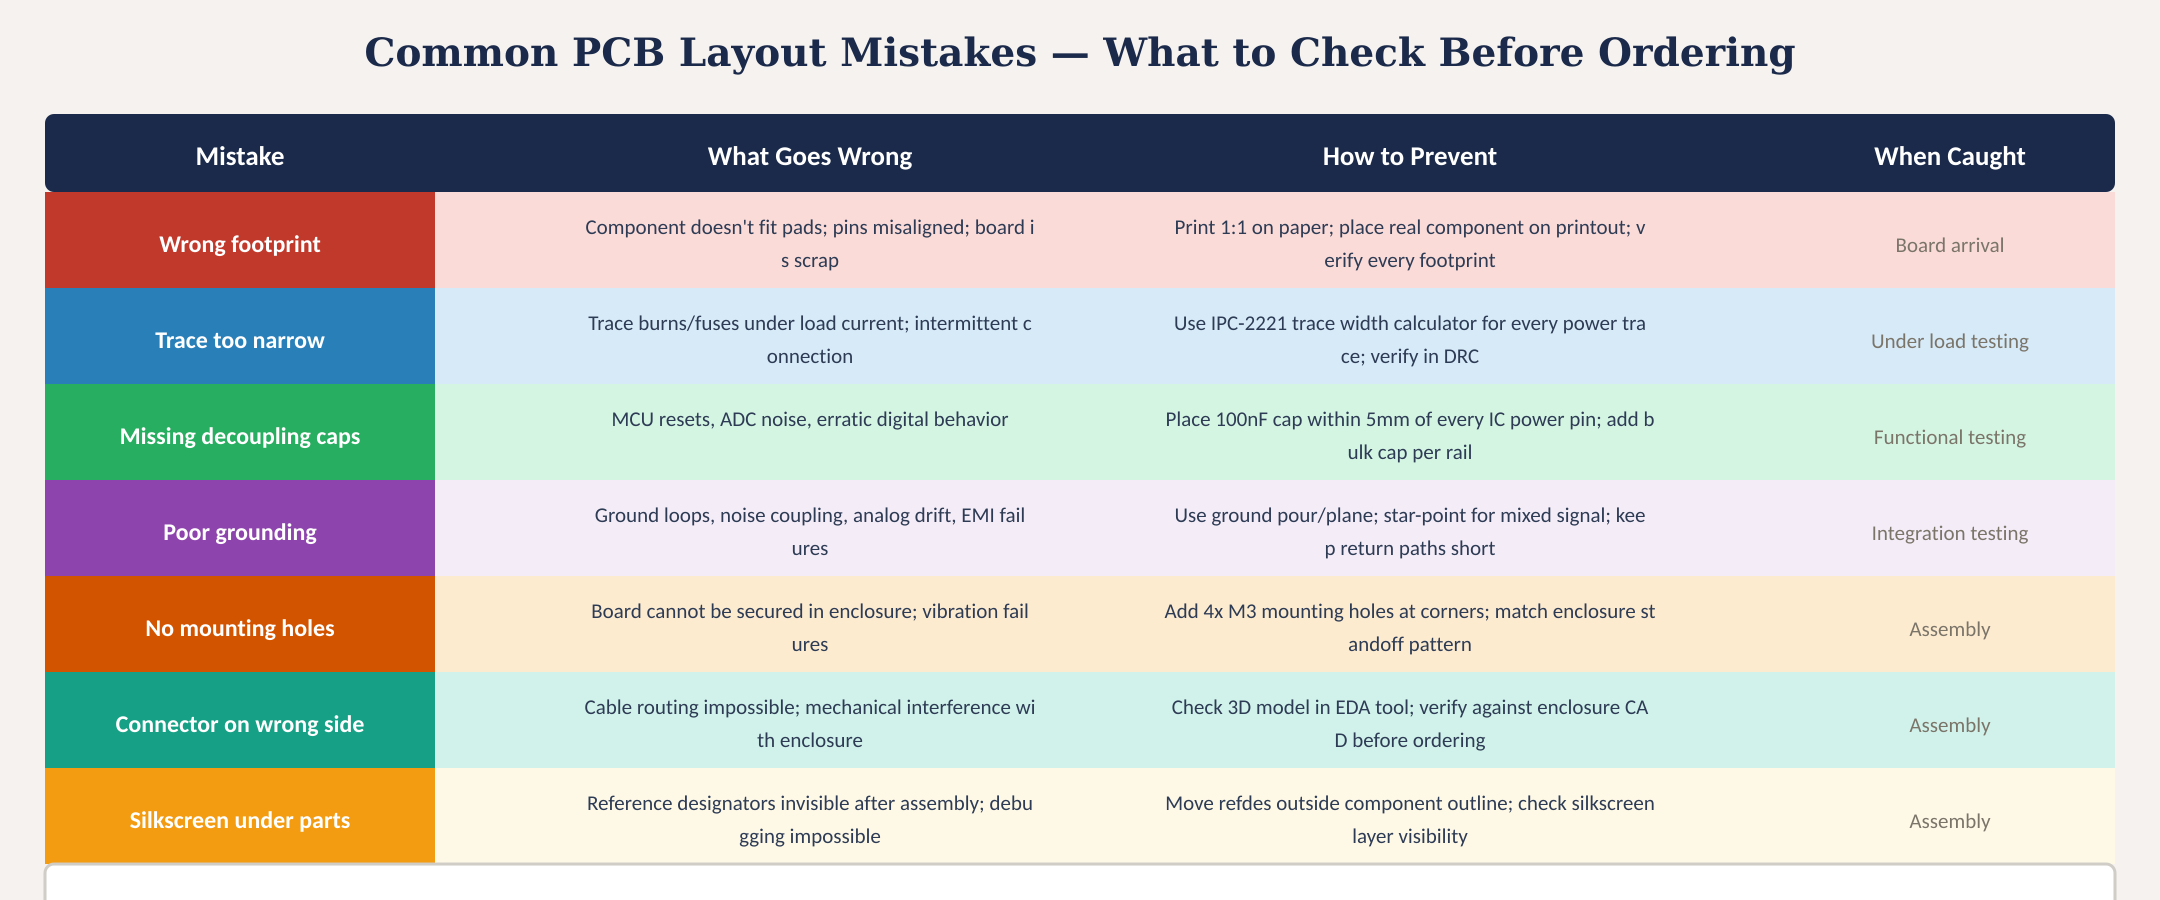
\includegraphics[width=\textwidth]{master_figs/fig_pcb_common_mistakes.png}
\caption{Seven common PCB layout mistakes with consequences and prevention strategies.}\label{fig:mistakes}
\end{figure}

Wrong footprint (scrap board), trace too narrow (burns under load), missing decoupling caps (erratic behavior), poor grounding (noise), no mounting holes (cannot secure board), connector on wrong side (cable routing impossible), silkscreen under parts (cannot read refdes). Prevention: print 1:1, run DRC, peer review, use 3D viewer.

\subsection{Development Boards vs Custom PCBs}
Use dev boards when: circuit is straightforward, form factor is not critical, timeline is tight, design is still evolving, or a suitable module already exists. Use custom PCBs when: specific form factor required, noise-sensitive analog, high reliability needed, multiple units, or clean cable routing. A well-wired dev board that meets requirements is superior to a custom PCB that delays the project.

\section{Artifact Handoff: What This Chapter Supports}
\begin{table}[htbp]\centering\small
\begin{tabularx}{\textwidth}{l X l}
\toprule
\textbf{Artifact} & \textbf{Description} & \textbf{Key Deliverable For} \\
\midrule
Schematic & Complete circuit with all component values & CDR, FDR \\
PCB Layout & Gerber files ready for fabrication & CDR (procurement) \\
BOM (electronics) & Components with package, value, vendor, Plan B & CDR, FDR \\
\bottomrule
\end{tabularx}
\end{table}

\section{PCB Design Rules for Student Projects}
\subsection{Trace Width and Current Capacity}
The PCB trace must be wide enough to carry the required current without excessive temperature rise. For external layers on 1\,oz copper (35\,$\mu$m thick):

\begin{itemize}[nosep,leftmargin=1.5em]
\item 0.25\,mm (10\,mil): 0.5\,A max (signal traces)
\item 0.5\,mm (20\,mil): 1.0\,A (low-power signals and buses)
\item 1.0\,mm (40\,mil): 2.0\,A (moderate power)
\item 2.5\,mm (100\,mil): 4.0\,A (motor drivers, heater connections)
\item 5.0\,mm (200\,mil): 7.0\,A (high-current power)
\end{itemize}

These values assume 10\,\degC{} temperature rise above ambient. For buried (internal) layers: derate by 50\%. For 2\,oz copper: multiply current capacity by $\sqrt{2} \approx 1.4$.

\begin{tipbox}[Use an Online IPC-2221 Calculator]
The lookup table above gives conservative approximations. For exact trace width calculations, use an online IPC-2221 calculator (search ``IPC-2221 trace width calculator''; Saturn PCB Toolkit is a popular free option). Enter your current, copper weight, allowable temperature rise, and ambient temperature to get a precise result. This is more accurate than a table and accounts for your specific conditions. For MEGN~301 projects, always round up to the next standard trace width and add 25\% margin on power traces.
\end{tipbox}

\subsection{Clearance and Creepage}
\textbf{Clearance}: the shortest distance through air between two conductors. For circuits under 50\,V: minimum 0.25\,mm (10\,mil). For 50--300\,V: minimum 1.5\,mm.

\textbf{Creepage}: the shortest distance along a surface between two conductors. Creepage must be larger than clearance because surface contamination (dust, flux residue, moisture) reduces the breakdown voltage. For circuits under 50\,V: minimum 0.5\,mm. For mains-connected circuits: consult IPC-2221 or the relevant safety standard.

\subsection{Via Design}\index{via (PCB)}
Vias connect traces between layers. For signal vias: 0.3\,mm drill, 0.6\,mm pad. For power vias: 0.4\,mm drill, 0.8\,mm pad, or use multiple vias in parallel for high current. Thermal vias under power components (voltage regulators, MOSFETs) connect the component pad to internal or bottom copper planes for heat dissipation. Use a grid of 4--9 vias with 0.3\,mm drill directly under the thermal pad.

\section{Component Placement Strategy}
Good placement is 80\% of good PCB design. Follow this sequence:

(1) \textbf{Place connectors first}: power input, signal I/O, programming header. These have fixed locations (edge of board, near panel cutouts). All other placement works around them.

(2) \textbf{Place the MCU}: central location, near the programming header. Orient so that bus signals (SPI, I2C, UART) route cleanly to their destinations.

(3) \textbf{Place power components}: voltage regulator near the power input connector. Input capacitor between the regulator and connector. Output capacitor between the regulator and the MCU. Keep the power path short and wide.

(4) \textbf{Place analog components}: sensors, amplifiers, ADCs as far as possible from switching noise sources (voltage regulators, motor drivers, digital buses). Ideally on the opposite side of the board or in a separate analog ground island.

(5) \textbf{Place remaining digital components}: group by function (communication, display, storage). Keep I2C devices on a clean bus with short traces.

\section{Design Review Before Fabrication}
Before submitting the PCB for fabrication, perform a systematic review:

\textbf{Schematic review}: verify every net is connected as intended. Check power and ground connections for every IC. Verify component values match the design calculations.

\textbf{Layout review}: run the DRC (Design Rule Check) and fix all violations. Visually inspect: are all traces routed? Are power traces wide enough? Are decoupling capacitors close to their ICs? Is there adequate clearance around mounting holes?

\textbf{3D review}: if the EDA tool supports 3D rendering (KiCad, Altium), verify that components do not interfere with the enclosure, connectors are accessible, and tall components do not block test points.

\textbf{Fabrication files}: generate Gerber files and the drill file. Open them in a Gerber viewer (KiCad's built-in viewer, or the fab house's online viewer) and verify that the actual output matches the design. Check that the board outline, mounting holes, and silkscreen are correct.
\begin{keyconceptbox}[Mandatory: 10$\times$ Visual Inspection Before Power-On]
Before applying power to any newly assembled PCB, perform a visual inspection under at least 10$\times$ magnification (jeweler's loupe, USB microscope, or stereo microscope). Inspect every solder joint for:

\textbf{Solder bridges}: unintended connections between adjacent pads, especially on fine-pitch ICs (0.5\,mm pitch QFP, 0.65\,mm SOIC). A single bridge between V$_{\text{CC}}$ and an I/O pin will destroy the IC at power-on.

\textbf{Cold joints}: dull, grainy, or blobby joints that did not wet properly. These create intermittent connections that work on the bench but fail under vibration.

\textbf{Tombstoned components}: 0402 and 0603 passives that lifted on one end during reflow, creating an open circuit. The component stands vertically like a tombstone\index{tombstoned component}.

\textbf{Missing components}: compare the board to the BOM and assembly drawing. A missing decoupling capacitor can cause oscillation; a missing pull-up resistor can hang the I2C bus.

\textbf{Polarity}: verify orientation of every polarized component (electrolytic capacitors, diodes, ICs, connectors). A reversed electrolytic capacitor will explode within seconds of power-on.

This inspection is a \textbf{gate}: no power is applied until a second team member has signed off on the visual inspection. This 5-minute check prevents the most common cause of PCB failure in student projects: immediate destruction of components due to assembly errors that were visible but unchecked.
\end{keyconceptbox}

\begin{quickrefbox}[Quick Reference: PCB Specifications for JLCPCB/PCBWay Student Orders]
\begin{table}[H]\centering\small
\begin{tabularx}{\textwidth}{l X}
\toprule
\textbf{Parameter} & \textbf{Typical Student Project Values} \\
\midrule
Layer count & 2-layer (default; 4-layer for mixed-signal or dense designs) \\
Copper weight & 1\,oz/ft$^2$ external (standard); 2\,oz for high-current ($>$3\,A) traces \\
Min trace/space & 6\,mil / 6\,mil (JLCPCB standard); use 10/10\,mil unless space-constrained \\
Min via drill/pad & 0.3\,mm drill / 0.6\,mm pad (standard); 0.2/0.45\,mm available \\
Trace width: 1\,A & $\geq$20\,mil (1-oz external copper, 10\,\degC{} rise) \\
Trace width: 3\,A & $\geq$50\,mil (1-oz) or $\geq$30\,mil (2-oz) \\
Decoupling cap placement & $\leq$5\,mm from IC power pin; via to ground plane directly under cap pad \\
Board thickness & 1.6\,mm (standard); 0.8\,mm for flexible mounting \\
Surface finish & HASL (cheapest), ENIG (flat pads, fine-pitch, \$2--5 extra) \\
Typical cost & \$2--7 for 5 boards (2-layer, $<$100$\times$100\,mm) \\
Lead time & 5--7 days (standard), 1--3 days (express, \$15--30 extra) \\
\bottomrule
\end{tabularx}
\end{table}
\end{quickrefbox}

\section{Practice Questions}
\begin{enumerate}[leftmargin=1.5em]
\item Your project has a motor driver that draws 3\,A peak. What is the minimum trace width for the motor power traces on a 2-layer board with 1-oz external copper? What width would you actually use and why?
\item A teammate's PCB layout has the 100\,nF decoupling capacitors placed 25\,mm from the MCU power pins ``because there was more room over there.'' Explain why this is a problem and what the correct placement is.
\item You receive your first PCB from JLCPCB. Describe the exact sequence of steps you follow before connecting the board to your system.
\item Your team is debating whether to design a custom PCB or use an Arduino Nano + sensor breakout boards. The project is a battery-powered environmental monitor that must fit inside a 60$\times$40$\times$25\,mm waterproof enclosure. Argue for or against a custom PCB with specific reasoning.
\item A 2-layer board has all signal traces on the top layer and a ground pour on the bottom. A teammate routes a high-current motor trace on the bottom layer, cutting through the ground pour. What problems will this cause and how should it be fixed?
\item Your schematic uses an LM1117-3.3 voltage regulator in an SOT-223 package to power an ESP32. The datasheet shows a thermal pad on the bottom. Your PCB layout connects the thermal pad to a small isolated copper island with no vias. Calculate the power dissipation at 5\,V input, 3.3\,V output, 300\,mA load, and explain why the current thermal design is inadequate.
\item You are designing a mixed-signal board with a 12-bit ADC reading a strain gauge (millivolt-level signal) and an H-bridge motor driver on the same PCB. Describe three specific layout strategies to prevent motor noise from corrupting the ADC readings.
\item Your team's KiCad DRC reports 47 ``courtyard overlap'' warnings. Your teammate dismisses them: ``It compiles fine, just ignore warnings.'' Explain why courtyard overlaps are serious and what physical problem they represent.
\end{enumerate}

\subsection{Answers}
\begin{enumerate}[leftmargin=1.5em]
\item From the IPC-2221 reference: 3\,A on 1-oz external copper requires approximately 100\,mil (2.5\,mm) trace width. In practice, use 150--200\,mil (3.8--5\,mm) to provide thermal margin, reduce voltage drop, and account for peak transients. Always add margin on power traces; the cost is board space, not money.
\item At 25\,mm, the trace inductance between the cap and the IC power pin negates the decoupling effect. High-frequency noise (MHz range) sees the inductance as a high impedance and is not filtered. The cap must be within 5\,mm with the shortest possible traces and a via directly to the ground plane. The loop area (VCC pin $\to$ cap $\to$ GND via $\to$ GND plane $\to$ IC GND pin) must be minimized.
\item Follow the six-step bring-up protocol: (1) Visual inspection under magnification for bridges, cold joints, and wrong-orientation parts. (2) Multimeter continuity check for VCC-to-GND shorts. (3) Current-limited bench supply at 50\,mA, apply expected voltage. (4) Measure all power rails with multimeter. (5) Increase current limit to operating level, monitor 60 seconds for heat/smell. (6) Load firmware, test basic I/O.
\item Argue FOR custom PCB: the 60$\times$40$\times$25\,mm enclosure is too small for an Arduino Nano (45$\times$18\,mm) plus breakout boards plus wiring. A custom board can integrate the MCU, sensors, and battery management into the available footprint with board-edge connectors for waterproof cable glands. The waterproof requirement also favors a single board with conformal coating over loose wiring that can vibrate and corrode. However: this requires the design to be frozen by CDR and 4--6 weeks of lead time.
\item The motor trace cuts the ground pour, forcing signal return currents to detour around the gap. This creates a large current loop that radiates EMI and couples noise into adjacent signal traces. The motor's switching noise (from PWM) will appear as voltage spikes on the ground plane near the gap, potentially corrupting ADC readings and causing MCU resets. Fix: route the motor power traces on the top layer using wide traces, keeping the bottom ground pour continuous. If the motor trace must cross to the bottom, use a narrow bridge with ground pour restored on both sides and stitching vias.
\item $P = (5.0 - 3.3) \times 0.3 = 0.51$\,W. SOT-223 $\theta_{JA}$ without thermal vias $\approx 150$\,\degC{}/W, so $\Delta T = 76.5$\,\degC{}. At 25\,\degC{} ambient: $T_J = 101.5$\,\degC{}, approaching the 125\,\degC{} limit. At 40\,\degC{} ambient (inside an enclosure): $T_J = 116.5$\,\degC{}, dangerous. The isolated copper island with no vias provides poor thermal coupling to inner layers. Fix: add an array of thermal vias (5--9 vias, 0.3\,mm drill, 1.0\,mm pitch) under the thermal pad, connecting to the ground plane on Layer~2. This reduces $\theta_{JA}$ to $\sim$60\,\degC{}/W.
\item (1) Physical separation: place ADC and strain gauge conditioning on the left half of the board, motor driver on the right, with a clear ``quiet zone'' boundary between them. (2) Separate analog supply: use an RC filter (10\,$\Omega$ + 10\,$\mu$F) between digital VCC and the ADC's AVCC pin to prevent motor switching noise from reaching the analog reference. (3) Guard ring/trace: surround the strain gauge signal traces with a grounded guard trace connected to the analog ground, shielding them from electric field coupling. Additionally: route motor power traces perpendicular (not parallel) to analog signal traces when crossings are unavoidable.
\item Courtyard overlaps mean two components occupy the same physical space on the board. They will either mechanically interfere (components crash into each other during assembly), or their solder pads will short together. DRC warnings are not cosmetic; they represent physical manufacturing problems. Fix: move one component until courtyards no longer overlap. If space is genuinely tight, verify in the 3D viewer that the components physically clear each other.
\end{enumerate}


